%This is a Latex file.
\documentclass[12pt]{article}
\usepackage{
	latexsym,
	fancyhdr,
	amsmath,
	amsfonts,
	dsfont,
	amsthm,
	amssymb,
	mathrsfs,
	mathtools
}
\usepackage[margin=0.94in]{geometry}
\usepackage{lastpage} % Required to determine the last page for the footer
\usepackage{tikz}
\usepackage{url, hyperref}

\parindent 0pt

\pagestyle{fancy} \lhead{\sf MTH 411} \chead{\sf Homework \#04}
\rhead{\sf Due: Friday 10/12/2018} \lfoot{} \cfoot{} \rfoot{}

\newcommand{\N}{\mathds{N}}
\newcommand{\Z}{\mathds{Z}}
\renewcommand{\vec}[1]{\overrightarrow{#1}}
\newcommand{\C}{\mathbb{C}}
\newcommand{\R}{\mathbb{R}}
\newcommand{\G}{\mathbb{G}}
\newcommand{\Q}{\mathbb{Q}}
\DeclarePairedDelimiter\abs{\lvert}{\rvert}

\begin{document}

{\bf Reading}: \fbox{Sections 6.}

\

{\bf Section 6 Problems}: \underline{You should be able to work out all problems}
%\begin{itemize}
%\item 
%\end{itemize}

\


\hrulefill

\

The following problems are {\bf due on 11:59pm Friday 10/12/2018}.  Submit both LaTeX and pdf files to the appropriate D2L Dropbox. 

Please name the files using the following format:
\begin{center}
\fbox{LastName$\_$FirstName$\_$MTH411$\_$Fall2018$\_$HW$\_$3}
\end{center}

You may discuss the problems with your classmates, but your write-up must be your own.  Any problems marked with an asterisk (*) denote problems you can not discuss with anyone except for me.\\

Please include the statements of the problems in your HW submissions. For any Extra problems you can copy the statements from the LaTeX file that generated this pdf. However, you will have to transcribe the remaining problems from Fraleigh.

\

\textbf{Section 6}: 9, 10, 14, 16, 18, 22, 24, 26, 27, 30, 33-37, 40, 49\\
Proofs: 45, 47, 55

%\textbf{Extras}:
%\begin{enumerate}
%\item
%\item
%\item
%\end{enumerate}
 \clearpage
\begin{enumerate}
	\item[6.09] Find the number of generators of a cyclic group of order 8 \\
		As all relatively prime solutions to $ \gcd(8,n) $ for $ 0 \leq n < 8 $ will result in the numbers that generate a cyclic group of order 8. Thus,there are 4 generators of a cyclic group of order 8, namely 1,2,5,7.
	\item[6.10] Find the number of generators of a cyclic group of order 12\\
			As all relatively prime solutions to $ \gcd(12,n) $ for $ 0 \leq n < 12 $ will result in the numbers that generate a cyclic group of order 8. Thus,there are 4 generators of a cyclic group of order 8, namely 1,5,7,11.
	\item[6.14] Find the number of automorphisms of $\Z_8$\\
		There are 4 automorphisms of $ \Z_8 $ as 1 can be taken to 1,3,5 and 7.
	
	\item[6.16] Find the number of automorphisms of $\Z_{12}$\\
				There are 4 automorphisms of $ \Z_{12} $ as 1 can be taken to 1,5,7 and 11.
	
	\item[6.18] Find the number of elements of the cyclic subgroup of $\Z_{42}$ generated by 30.\\
	As $ \gcd(42,30)=6 $ and $ \frac{42}{6}=7, \langle 30 \rangle $ has 7 elements.
	
	\item[6.22] Find all subgroups of $\Z_{12}$ and draw the subgroup diagram for the subgroup.
	
	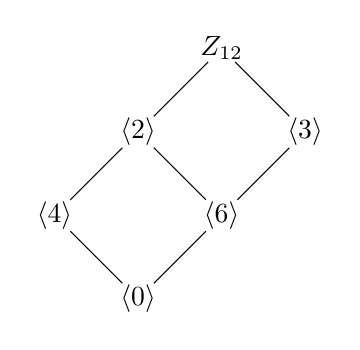
\begin{tikzpicture}[node distance=1.5cm]
	\title{Subgroup diagram for $\Z_{12}$}
	\node(12)                 {$\Z_{12}$};
	\node(2)       [below left of=12] {$\langle2\rangle$};
	\node(3)      [below right of=12]  {$\langle3\rangle$};
	
	\node(6)      [below left of=3]       {$\langle6\rangle$};
	\node(0)      [below left of=6]       {$\langle0\rangle$};
	\node(4)      [below left of=2]  {$\langle4\rangle$};
	
	\draw [shorten <=-4pt, shorten >= -4pt] (12)       -- (2);
	\draw[shorten <=-4pt, shorten >= -4pt](12)       -- (3);
	\draw [shorten <=-4pt, shorten >= -4pt](3)       -- (6);
	\draw [shorten <=-4pt, shorten >= -4pt](6)       -- (0);
	\draw [shorten <=-4pt, shorten >= -4pt](2)       -- (6);
	\draw [shorten <=-4pt, shorten >= -4pt](4)      --(2);
	\draw [shorten <=-4pt, shorten >= -4pt](4)      --(0);
	
	
	
	
	\end{tikzpicture}
	
	\item[6.24] Find all subgroups of $\Z_8$ and draw the subgroup diagram for the subgroup.
	
	\begin{tikzpicture}[node distance=1cm]
	\title{Subgroup diagram for $\Z_{8}$}
	\node(8)                 {$\Z_{8}$};
	\node(2)       [below of=12] {$\langle2\rangle$};
	\node(4)      [below of=2]  {$\langle4\rangle$};
	\node(0)      [below of=4]       {$\langle0\rangle$};
	
	
	
	\draw [shorten <=-2pt, shorten >= -2pt](8)       -- (2);
	\draw [shorten <=-2pt, shorten >= -2pt](4)       -- (2);
	\draw [shorten <=-2pt, shorten >= -2pt](4)       -- (0);
	
	\end{tikzpicture}
	
	\item[6.26] Find all orders of subgroups of $\Z_8$.\\
		By the previous exercise we know the subgroups of $ \Z_8 $. Thus, $ \Z_8 $ has subgroups of order 1,2,4, and 8.
	
	\item[6.27] Find all orders of subgroups of $\Z_{12}$.\\
				By the previous exercise we know the subgroups of $ \Z_{12} $. Thus, $ \Z_{12} $ has subgroups of order 1,2,3,4,6 and 12.
	\item[6.30] Correct the definition if needed. An element $a$ of a group $G$ has $\textit{order } n\in \Z^+$ if and only if $a^n = e$.\\
	An element $a$ of a group $G$ has $\textit{order } n\in \Z^+$ if and only if $a^n = e$ and $ n $ is the smallest positive integer for which this equation is true.
	
	\item[6.33-6.37]Either give an example, or show why there exists no example.
	
	\item[6.33] A finite group that is not cyclic.\\
		The Klein 4-group
	\item[6.34] An infinite group that is not cyclic.\\
		$ \langle \R , + \rangle $
	\item[6.35] A cyclic group having only one generator.\\
		$ \Z_2 $
	
	\item[6.36] An infinite cyclic group having four generators.\\
		No example exists. As every infinite cyclic group is isomorphic to $ \rangle \Z,+\langle $ which only has two generators, 1 and -1.
	
	\item[6.37] A finite group having four generators.\\
	$ \Z_8 $
	\item[6.40] Find the primitive nth roots of unity for $n = 8$.\\
	 As $U_8$ is isomorphic to $Z_8$, we know the generators of $Z_8$ are isomorphic to the generators of $U_8$. Thus, the primitive 8th roots of unity are $\zeta, \zeta^3, \zeta^5, \zeta^7$
	
	\item[6.49] Show by a counterexample that the following "converse" of Theorem 6.6 is not a theorem: "If a group $G$ is such that every proper subgroup is cyclic, then $G$ is cyclic."\\
	The Klein 4 group is a counter example as every proper subgroup is cyclic, but the group itself is not cyclic.
	\item[6.45] Let $r$ and $s$ be positive integers. Show that $H=\{nr+ms|n,m \in \Z \}$ is a subgroup of $\Z$\\
		Let $ a,b \in H $. Then, for some $n_1,m_1 \in \Z, a = n_1r+m_1s $ and  for some $n_2,m_2 \in \Z, b = n_2r+m_2s $. Notice. 
		\[n_1r+m_1s+n_2r+m_2s=(n_1+n_2)r+(m_1+m_2)s\]
		shows that the set is closed under addition.\\
		\\
		As $ 0r+0s=0 $, we see that 0 is in the set.\\
		\\
		Let $ a = nr+ms \in H$ we have that \[-a=-(nr+ms)=-nr-ms=(-n)r+(-m)s\]
		and therefore $ -a\in H $\\
		Therefore, $ H \leq \Z $
	\item[6.47] Let $r$ and $s$ be positive integers.
	\begin{enumerate}
		\item Define the \textbf{least common multiple} of $r$ and $s$ as a generator of a certain cyclic group.\\
		As a subgroup of the cyclic group $ \langle\Z, +\rangle$, the subgroup $G = r\Z \cap s\Z$ is cyclic. The positive generator of $ G $ is the least common multiple of $ r  $and$  s $
		\item Under what condition is the least common multiple of $r$ and $s$ their product, $rs$?\\
		When $ r $ and $ s $ are relatively prime, the lcm of $ r $ and $ s $ is their product, $ rs $ 
		\item Generalizing part $(b)$, show that the product of the greatest common divisor and of the least common multiple of $r$ and $s$ is $rs$.\\
		
		 Let $ i,j,k,q\in\Z $, $ \gcd(r,s) = d = ir + js $ ,and lcm$(r,s) = m = kr = qs$. Notice.
		 \[md = mir + mjs = qsir + krjs = (qi + kj)rs\], thus $ rs $ is a divisor of $ md $. Now let $ u,v\in\Z$. Let $ r = ud $
		and $  s = vd$. Then $ rs = uvdd = (uvd)d $, and $ uvd = rv = su $ is a multiple of $ r $ and $ s $. Then,  $ uvd = mt $. Thus,$  rs = mtd = (md)t, $ so $ md $ is divisor of $ rs $. Therefore, $ md = rs.$
		
	\end{enumerate}
	
	\item[6.55] Show that $ \Z_p $ has no proper nontrivial subgroups if $ p $ is a prime number.\\
		All positive integers less than $ p $ are relatively prime to $ p $ as $ p $ is prime. Thus, they all generate $ \Z_p $. Therefore, $ Z_p $ has no proper cyclic subgroups, and by definition of being cyclic, $ \Z_p $ has only cyclic subgroups. Therefore, $ \Z_p $ has no proper nontrivial subgroup.
	\end{enumerate}
\end{document}
